\documentclass{article}

\usepackage{graphicx}
\usepackage{tikz}
\usepackage{tikzsymbols}
\usetikzlibrary{calc,patterns,shapes.geometric}
\pagestyle{empty}
\usepackage[margin=0pt]{geometry}
\geometry{papersize={14in,12in}}

\def\centerarc[#1](#2)(#3:#4:#5){\draw[#1] ($(#2)+({#5*cos(#3)},{#5*sin(#3)})$) arc (#3:#4:#5);}

\begin{document}
	\begin{figure}
		\centering
		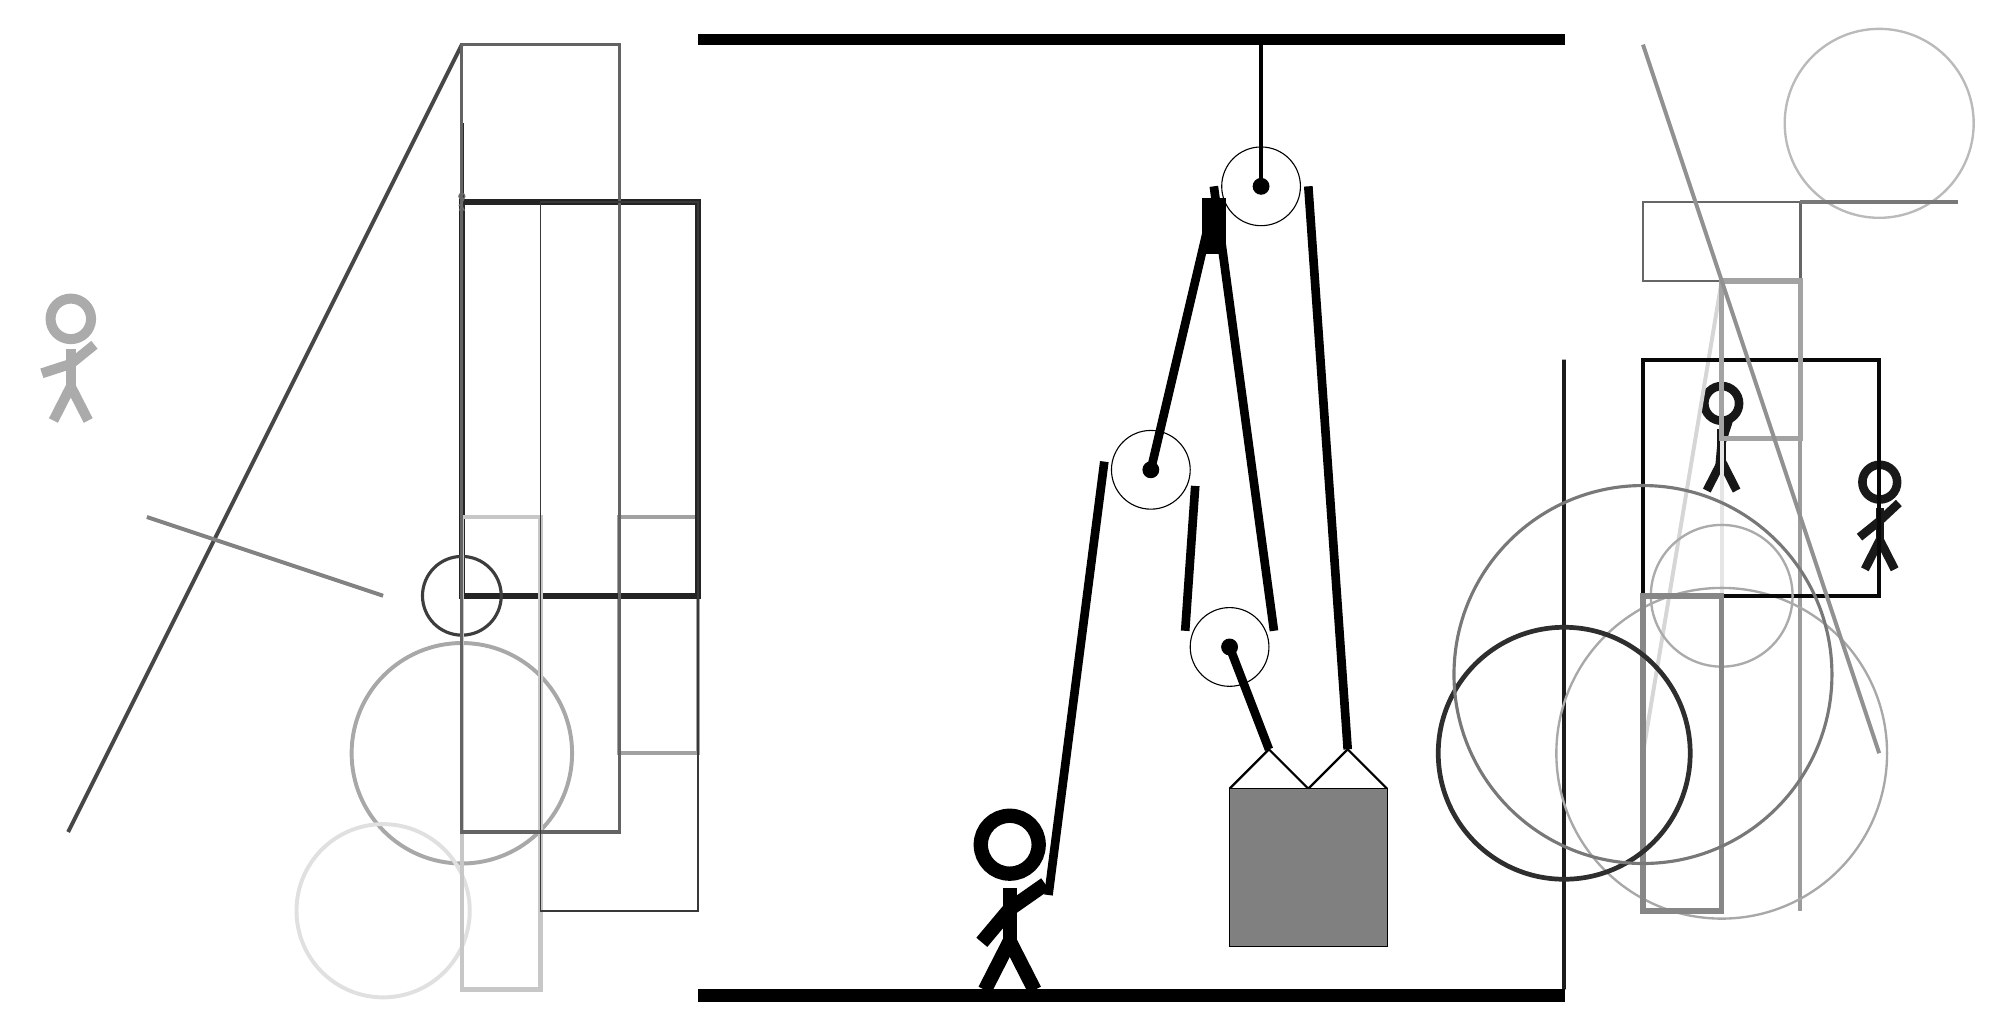
\begin{tikzpicture}
			%%%%% START %%%%%
			
			\draw[fill=black] (-6, 9) rectangle (5, 9.125);
			
			\draw (-0.25, 3.6) circle (0.5);
			\draw[fill=black] (-0.25, 3.6) circle (0.1);
			
			\draw (0.75, 1.35) circle (0.5);
			\draw[fill=black] (0.75, 1.35) circle (0.1);
			
			\draw (1.15, 7.2) circle (0.5);
			\draw[fill=black] (1.15, 7.2) circle (0.1);
			\draw[very thick] (1.15, 7.2) -- (1.15, 9);
			
			\draw[thick]  (0.75, -0.45) -- (1.25, 0.05) -- (1.75, -0.45) -- (2.25, 0.05) -- (2.75, -0.45);
			\draw[fill=black!50] (0.75, -0.45) rectangle (2.75, -2.45);
			
			\node[line width=0.7mm, color=black!90] at (9, 3) {\Strichmaxerl[6][39][43]};
			
			\draw [line width=0.3mm, color=black!27](9, 8) circle (1.2);
			\draw[line width=0.5mm, color=black!39](8, -2) -- (8, 4);
			\node[line width=0.5mm, color=black!91] at (7, 4) {\Strichmaxerl[6][85][72]};
			
			\draw[line width=0.5mm, color=black!10](7, 2) -- (7, 5);
			\draw[line width=0.5mm, color=black!37] (-6, 0) rectangle (-7, 3);
			\draw[line width=0.5mm, color=black!72](-9, 9) -- (-14, -1);
			\draw [line width=0.5mm, color=black!34](-9, 0) circle (1.4);
			\draw[line width=0.5mm, color=black!89] (5, -3) rectangle (5, 5);
			\draw[line width=0.7mm, color=black!86] (-6, 7) rectangle (-9, 2);
			\draw[line width=0.5mm, color=black!16](6, 0) -- (7, 6);
			\draw[line width=0.3mm, color=black!60] (6, 7) rectangle (8, 6);
			\draw[line width=0.5mm, color=black!84](-9, 6) -- (-9, 8);
			\draw[line width=0.5mm, color=black!49](-10, 2) -- (-13, 3);
			\draw [line width=0.4mm, color=black!76](-9, 2) circle (0.5);
			\node[line width=0.4mm, color=black!33] at (-14, 5) {\Strichmaxerl[7][18][39]};
			
			\draw [line width=0.3mm, color=black!34](7, 0) circle (2.1);
			\draw[line width=0.5mm, color=black!97] (6, 2) rectangle (9, 5);
			\draw [line width=0.5mm, color=black!12](-10, -2) circle (1.1);
			
			\draw[line width=0.6mm, color=black!22] (-8, -3) rectangle (-9, 3);
			\draw[line width=0.4mm, color=black!61] (-7, -1) rectangle (-9, 9);
			
			\draw [line width=0.3mm, color=black!33](7, 2) circle (0.9);
			
			\draw[line width=0.7mm, color=black!47] (6, 2) rectangle (7, -2);
			\draw[line width=0.2mm, color=black!78] (-6, -2) rectangle (-8, 7);
			\draw[line width=0.7mm, color=black!36] (7, 6) rectangle (8, 4);
			
			\draw [line width=0.6mm, color=black!82](5, 0) circle (1.6);
			\node[line width=0.7mm, color=black!59] at (-9, 7) {\Strichmaxerl[1][49][63]};
			\draw [line width=0.4mm, color=black!53](6, 1) circle (2.4);
			\draw[line width=0.5mm, color=black!53](10, 7) -- (8, 7);
			
			\draw[line width=0.5mm, color=black!43](6, 9) -- (9, 0);
			
			\draw[line width=1.1mm] (-0.25, 3.6) -- (0.55, 7.0);
			\draw[line width=1.1mm, fill=black](0.45, 6.4) rectangle (0.65, 7.0);
			\draw[line width=1.1mm] (-1.55, -1.8) -- (-0.8409, 3.7042);
			\centerarc[line width=1.1mm](-0.25, 3.6)(-20:170:0.6);
			\draw[line width=1.1mm] (0.3138, 3.3948) -- (0.1862, 1.5552);
			\centerarc[line width=1.1mm](0.75, 1.35)(160:380:0.6);
			\draw[line width=1.1mm] (1.3138, 1.5552) -- (0.55, 7.2);
			\draw[line width=1.1mm](0.75, 1.35) -- (1.25, 0.05);
			\centerarc[line width=1.1mm](1.15, 7.2)(0:180:0.6);
			\draw[line width=1.1mm] (1.75, 7.2) -- (2.25, 0.05);
			
			\node at (-2, -1.9) {\Strichmaxerl[10][50][35]};
			
			\draw[fill=black] (-6, -3) rectangle (5, -3.15);
			
			%%%%% END %%%%%
		\end{tikzpicture}
	\end{figure}	
\end{document}